\documentclass[10pt,letterpaper,notitlepage]{article}
\usepackage[utf8]{inputenc}
\usepackage{amsmath}
\usepackage{amsfonts}
\usepackage{amssymb}
\usepackage{graphicx}
\usepackage{cancel}
\usepackage{float}
\usepackage{cite}

\usepackage[ruled,vlined]{algorithm2e}


\usepackage[left=0.75in, right=0.75in, bottom=1.0in,top=0.75in]{geometry}

%\usepackage{caption} 
%\captionsetup[table]{skip=10pt}
%\usepackage[font=small,labelfont=bf]{caption}

\usepackage{comment}
\usepackage{listings}

\usepackage{color}
\definecolor{Brown}{cmyk}{0,0.81,1,0.60}
\definecolor{OliveGreen}{cmyk}{0.64,0,0.95,0.40}
\definecolor{CadetBlue}{cmyk}{0.62,0.57,0.23,0}

\usepackage{multicol}

\usepackage{appendix}

\usepackage{fancyhdr}
%\usepackage[colorlinks=true,linkcolor=blue,urlcolor=black,bookmarksopen=true,bookmarks]{hyperref}
\usepackage{bookmark}


%============================= Put document title here
\newcommand{\DOCTITLE}{Gauss Elimination programming assignment}  

%=============================  Load list of user-defined commands
% Mark URL's
\newcommand{\URL}[1]{{\textcolor{blue}{#1}}}
%
% Ways of grouping things
%
\newcommand{\bracket}[1]{\left[ #1 \right]}
\newcommand{\bracet}[1]{\left\{ #1 \right\}}
\newcommand{\fn}[1]{\left( #1 \right)}
\newcommand{\ave}[1]{\left\langle #1 \right\rangle}
\newcommand{\norm}[1]{\Arrowvert #1 \Arrowvert}
\newcommand{\abs}[1]{\arrowvert #1 \arrowvert}
%
% Derivative forms
%
\newcommand{\dxdy}[2]{\frac{\partial #1}{\partial #2}}
\newcommand{\dxy}[2]{\frac{d #1}{d #2}}
\newcommand{\dydx}[1]{\frac{\partial #1}{\partial x}}
\newcommand{\dydt}[1]{\frac{\partial #1}{\partial t}}
\newcommand{\dxdz}[1]{\frac{\partial #1}{\partial z}}
\newcommand{\dfdt}[1]{\frac{\partial}{\partial t} \fn{#1}}
\newcommand{\dfdz}[1]{\frac{\partial}{\partial z} \fn{#1}}
\newcommand{\ddt}[1]{\frac{\partial}{\partial t} #1}
\newcommand{\ddz}[1]{\frac{\partial}{\partial z} #1}
\newcommand{\dd}[2]{\frac{\partial}{\partial #1} #2}
\newcommand{\ddx}[1]{\frac{\partial}{\partial x} #1}
\newcommand{\ddy}[1]{\frac{\partial}{\partial y} #1}
\newcommand{\dxdyn}[3]{\frac{\partial ^{#3} #1 }{\partial #2 ^{#3}}}
\newcommand{\Dxdy}[2]{\frac{D #1}{D #2}}
\newcommand{\Dxy}[2]{\frac{D #1}{D #2}}
%
% Bold quantities
% 
\newcommand{\Omegabf}{\mathbf{\Omega}}
\newcommand{\bnabla}{\boldsymbol{\nabla}}
\newcommand{\position}{\mathbf{x}}
\newcommand{\dotp}{\boldsymbol{\cdot}}
%
% Vector forms
%
\renewcommand{\vec}[1]{\mbox{$\stackrel{\longrightarrow}{#1}$}}
\renewcommand{\div}{\mbox{$\vec{\mathbf{\nabla}} \cdot$}}
\newcommand{\grad}{\mbox{$\vec{\mathbf{\nabla}}$}}
\newcommand{\bb}[1]{\bar{\bar{#1}}}
%
% Vector forms boldfaced
\newcommand{\bvec}[1]{\mathbf{#1}}
\newcommand{\bdiv}{\boldsymbol{\nabla} \boldsymbol{\cdot}}
\newcommand{\bgrad}{\bnabla}
\newcommand{\mat}[1]{\bar{\bar{#1}}}
%
%
% Equation beginnings and endings
%
% Un-numbered equation with alignment
\newcommand{\beq}{\begin{equation*} \begin{aligned}}
\newcommand{\eeq}{\end{aligned}\end{equation*}}
% Numbered equation with alignment
\newcommand{\beqn}{\begin{equation}\begin{aligned}}
\newcommand{\eeqn}{\end{aligned}\end{equation}}  

% Numbered equation array, aligned	
\def\bea#1\eea{\begin{align}#1\end{align}}

\newcommand{\beas}{\begin{eqnarray*}}
\newcommand{\eeas}{\end{eqnarray*}}
\newcommand{\bdm}{\begin{displaymath}}
\newcommand{\edm}{\end{displaymath}}
%
% Equation punctuation
%
\newcommand{\pec}{\, ,}
\newcommand{\pep}{\, .} 
\newcommand{\pev}{\hspace{0.25in}}
%
% Equation labels and references, figure references, table references
%
\newcommand{\lequ}[1]{\label{eq:#1}}
\newcommand{\equ}[1]{Eq.~(\ref{eq:#1})}
\newcommand{\equs}[1]{Eqs.~(\ref{eq:#1})}
\newcommand{\requ}[1]{(\ref{eq:#1})}
\newcommand{\lfig}[1]{\label{fi:#1}}
\newcommand{\fig}[1]{Fig.~\ref{fi:#1}}
\newcommand{\figs}[1]{Figs.~\ref{fi:#1}}
\newcommand{\rfig}[1]{\ref{fi:#1}}
\newcommand{\lta}[1]{\label{ta:#1}}
\newcommand{\ta}[1]{Table~\ref{ta:#1}}
\newcommand{\rta}[1]{\ref{ta:#1}}
\newcommand{\lsec}[1]{\label{sec:#1}}
\newcommand{\rsec}[1]{\ref{sec:#1}}
%
% Superscript and subscript in text
%
\newcommand{\supertext}[1]{\ensuremath{^{\textrm{#1}}}}
\newcommand{\subtext}[1]{\ensuremath{_{\textrm{#1}}}}
%
% List beginnings and endings
%
\newcommand{\bl}{\bss\begin{itemize}}
\newcommand{\el}{\vspace{-.5\baselineskip}\end{itemize}\ess}
\newcommand{\ben}{\bss\begin{enumerate}}
\newcommand{\een}{\vspace{-.5\baselineskip}\end{enumerate}\ess}
%
% Figure and table beginnings and endings
%
\newcommand{\bfg}{\begin{figure}}
\newcommand{\efg}{\end{figure}}
\newcommand{\bt}{\begin{table}}
\newcommand{\et}{\end{table}}
%
% Tabular and center beginnings and endings
%
\newcommand{\bc}{\begin{center}}
\newcommand{\ec}{\end{center}}
\newcommand{\btb}{\begin{center}\begin{tabular}}
\newcommand{\etb}{\end{tabular}\end{center}}
%
% Single space command
%
\newcommand{\bss}{\begin{singlespace}}
\newcommand{\ess}{\end{singlespace}}
%
% Quick commands for symbols
%
\newcommand{\half}{\frac{1}{2}}
\newcommand{\third}{\frac{1}{3}}
\newcommand{\twothird}{\frac{2}{3}}
\newcommand{\fourth}{\frac{1}{4}}
\newcommand{\sixth}{\frac{1}{6}}
\newcommand{\mdot}{\dot{m}}
%\newcommand{\ten}[1]{\times 10^{#1}\,}
\newcommand{\cL}{{\cal L}}
\newcommand{\cD}{{\cal D}}
\newcommand{\cF}{{\cal F}}
\newcommand{\cE}{{\cal E}}
\renewcommand{\Re}{\mbox{Re}}
\newcommand{\Ma}{\mbox{Ma}}
\newcommand{\mA}{\mathbf{A}}
\newcommand{\mB}{\mathbf{B}}
\newcommand{\mC}{\mathbf{C}}
\newcommand{\E}{\mathcal{E}}
\newcommand{\F}{\mathcal{F}}
\newcommand{\Q}{\mathcal{Q}}
\newcommand{\U}{\mathbf{U}}
\renewcommand{\H}{\mathbf{H}}
\newcommand{\R}{\mathbf{R}}
\newcommand{\SN}{S$_{n}\,$}
\newcommand{\Flux}{\mathbf{F}}
\newcommand{\dt}{\Delta t}
\newcommand{\dx}{\Delta x}
\newcommand{\iL}{_{i,L}}
\newcommand{\iR}{_{i,R}}
\newcommand{\sa}{\sigma_a}
\newcommand{\sigsL}{\frac{\sigma_{s,i,L}^k}{2}}
\newcommand{\sigsR}{\frac{\sigma_{s,i,R}^k}{2}}
\newcommand{\sigtL}{\sigma_{t,i,L}^k}
\newcommand{\sigtR}{\sigma_{t,i,R}^k}
\newcommand{\halfh}{\frac{h_i}{2}}
\newcommand{\CN}[3]{\half\left[#1\right]^#2 + \half\left[#1\right]^#3}
\newcommand{\CNN}[3]{\half\left[#1\right]^#2 - \half\left[#1\right]^#3}
\newcommand{\BDF}[4]{\sixth\left[#1\right]^{#2} + \sixth\left[#1\right]^{#3} + \twothird\left[#1\right]^{#4}}
%
% More Quick Commands
%
\newcommand{\bi}{\begin{itemize}}
\newcommand{\ei}{\end{itemize}}
\newcommand{\dxi}{\Delta x_i}
\newcommand{\dyj}{\Delta y_j}
\newcommand{\ts}[1]{\textstyle #1}

\newcommand{\jcr}[1]{\textcolor{magenta}{#1}}
\usepackage[normalem]{ulem}
\newcommand{\ssout}[1]{\sout{\textcolor{magenta}{#1}}}

%
% Code syntax highlighting
%
%\lstset{language=C++,frame=ltrb,framesep=2pt,basicstyle=\linespread{0.8} \small,
%	keywordstyle=\ttfamily\color{OliveGreen},
%	identifierstyle=\ttfamily\color{CadetBlue}\bfseries,
%	commentstyle=\color{Brown},
%	stringstyle=\ttfamily,
%	showstringspaces=true,
%	tabsize=2,}

\lstset{language=C++,frame=ltrb,framesep=8pt,basicstyle=\linespread{0.8} \Large,
commentstyle=\ttfamily\color{OliveGreen},
keywordstyle=\ttfamily\color{blue},
identifierstyle=\ttfamily\color{CadetBlue}\bfseries,
stringstyle=\ttfamily,
tabsize=2,
showstringspaces=false,
numbers=left,
captionpos=t}

\renewcommand{\lstlistingname}{\textbf{Code Snippet}}% Listing -> Code Snippet


\begin{document}
\noindent
{\LARGE\textbf{\DOCTITLE}}
\newline
\newline
\newline
\noindent
{\Large Jan I.C. Vermaak$^{1,2}$}
\newline
\noindent\rule{\textwidth}{1pt}
{\small $^1$Center for Large Scale Scientific Simulations, Texas A\&M Engineering Experiment Station, College Station, Texas, USA.}
\newline\noindent
{\small $^2$Nuclear Engineering Department, Texas A\&M University, College Station, Texas, USA.}
\newline
\newline
\textbf{Abstract:}\newline\noindent
Gauss elimination (GE) forms the basis of many direct solvers. In this assignment we explore the definition of routines that can help us solve linear systems of equations, with all the routines based on either GE-itself or some variant, i.e., the Tri-diagonal Matrix Algorithm (TDMA) or general banded matrix solvers.
\newline
\newline\noindent
{\small
\textbf{Keywords:} gauss elimination, tri-diagonal matrix, banded matrix solvers}

\section{Introduction}
In C++ we can define a dense matrix and a vector in the following format:
\begin{verbatim}
typedef std::vector<double> Vec;
typedef std::vector<Vec> Mat;

Mat A(100,Vec(100,0.0));
Mat b(100,0.0);
\end{verbatim}

\noindent
For this case, we defined the matrix to be of dimension $100{\times}100$ and is initially zero. The vector $b$ is of dimension $100{\times}1$ and is also zero. If the matrix is filled with entries then we can define the most rudimentary solution of a system
$$
Ax = b
$$ 
as
$$
x = A^{-1}b
$$

\noindent
Gauss Elimination is the most fundamental algorithm to solve for $x$.

\section{Gauss Elimination without pivoting}

\begin{algorithm}
\caption{Gauss elimination without pivoting}
Forward elimination:\\
\For{$j=0; \ j < N-1; \ {++}j$}
{
	\For{$i=j+1; \ i < N; \ {++i}$}
	{
		$c = \frac{a_{ij}}{a_{jj}}$\\
		\For{$k=0; \ k < N; \ {++k}$}
		{
			$a_{ik} = a_{ik} - c a_{jk}$
		} 
	}
}
Back substitution:\\
\For{$i=N-1; \ i>=0; \ {--}i$}
{
	$S = b_i$\\
	\For{$j=i+1; \ j < N; \ {++}j$}
	{
		$S = S - a_{ij}x_j$
	}
	$x_i = \frac{S}{a_{ii}}$
}
\end{algorithm}

\noindent
The algorithm has two parts, a forward elimination part and a back-substitution part. The forward elimination step involves choosing a column $j$ for which to eliminate all the values below the diagonal. Each row $i$, where $i=j+1$, then subtracts from itself $c$ times the row above it (i.e. row $j$). The factor $c$ is chosen such that entry $a_{ji}$ becomes zero. The forward elimination process is graphically shown below.

\beq
\begin{bmatrix}
	a_{00} & a_{01} & a_{02} \\
	a_{10} & a_{11} & a_{12} \\
	a_{20} & a_{21} & a_{22} \\
\end{bmatrix}
\begin{bmatrix}
	x_0 \\ x_1 \\ x_2
\end{bmatrix}
=
\begin{bmatrix}
	b_0 \\ b_1 \\ b_2
\end{bmatrix}
\eeq 

\beq
\begin{matrix}
	\dots\\
	\text{row}_1 = \text{row}_1 - \frac{a_{10}}{a_{00}} \text{ row}_0\\
	\dots
\end{matrix}
\begin{bmatrix}
	a_{00} & a_{01} & a_{02} \\
	0    & a_{11}^1 & a_{12}^1 \\
	a_{20} & a_{21} & a_{22} \\
\end{bmatrix}
\begin{bmatrix}
	x_0 \\ x_1 \\ x_2
\end{bmatrix}
=
\begin{bmatrix}
	b_0 \\ b_1^1 \\ b_2
\end{bmatrix}
\eeq  

\beq
\begin{matrix}
	\dots\\
	\dots\\
	\text{row}_2 = \text{row}_2 - \frac{a_{20}}{a_{00}} \text{ row}_0
\end{matrix}
\begin{bmatrix}
	a_{00} & a_{01} & a_{02} \\
	0    & a_{11}^1 & a_{12}^1 \\
    0     & a_{21}^2 & a_{22}^2 \\
\end{bmatrix}
\begin{bmatrix}
	x_0 \\ x_1 \\ x_2
\end{bmatrix}
=
\begin{bmatrix}
	b_0 \\ b_1^1 \\ b_2^2
\end{bmatrix}
\eeq  

\beq
\begin{matrix}
	\dots\\
	\dots\\
	\text{row}_2 = \text{row}_2 - \frac{a_{21}}{a_{11}} \text{ row}_1
\end{matrix}
\begin{bmatrix}
	a_{00} & a_{01} & a_{02} \\
	0    & a_{11}^1 & a_{12}^1 \\
	0     & 0            & a_{22}^3 \\
\end{bmatrix}
\begin{bmatrix}
	x_0 \\ x_1 \\ x_2
\end{bmatrix}
=
\begin{bmatrix}
	b_0 \\ b_1^1 \\ b_2^3
\end{bmatrix}
\eeq  
\newline
\newline
The superscripts on $a$ here just denote the value of $a$ after a step. The second part of the algorithm is just simple back substitution.

\section{The Tri-diagonal matrix algorithm (TDMA)}
Also known as the Thomas algorithm. The algorithm assumes the system in the following form
\beq
\begin{bmatrix}
b_0 & c_0 &  &  & 0 \\
a_1 & b_1 & c_1    &  & \vdots \\
 & a_2 & b_2 & \ddots &\\
 & & \ddots & \ddots & c_{N-2} \\
 0 & & & a_{N-1} & b_{N-1}
\end{bmatrix}
\begin{bmatrix}
x_0 \\ x_1 \\ x_2 \\ \vdots \\ x_{N-1}
\end{bmatrix}
=
\begin{bmatrix}
d_0 \\ d_1 \\ d_2 \\ \vdots \\ d_{N-1}
\end{bmatrix}
\eeq 

\begin{algorithm}
\caption{The tri-diagonal matrix algorithm}
\textbf{Require}: $\vec{a}, \vec{b}, \vec{c}, \vec{d}$\\
\For{$i=1; \ i < N; \ {++}i$}
{
	$w = \dfrac{a_i}{b_{i-1}}$\\
	$b_i = b_i - w c_{i-1}$\\
	$d_i = d_i - w d_{i-1}$\\
}
$x_{N-1} = \dfrac{d_{N-1}}{b_{N-1}}$\\
\For{$i=N-2; \ i \ge 0; \ {--}i$}
{
	$x_i = \dfrac{(d_i - c_i x_{i+1})}{b_i}$
}
\end{algorithm}

\newpage
\section{Assignment}
\textbf{Part 1}. Write a c++ function that performs Gauss Elimination. The function needs to have the following signature:

\begin{verbatim}
typedef std::vector<double> Vec;
typedef std::vector<Vec> Mat;

Vec GaussElimination(const Mat& A, const Vec& b);
\end{verbatim}

Details:
\begin{itemize}
	\item The matrix $A$ and vector $b$ is passed as a constant reference, so they cannot be modified. Make an internal copy of $A$ and $b$.
	\item The function needs to return a new vector $x$.
	\item The function can deduce the size of the system, $N$, from the number of rows
	in the matrix but it should check that this is the same as the number of elements in $b$. If it is not then an error message needs to be printed and the program should quite using 
	\begin{verbatim}
		//print message then...
		exit(EXIT_FAILURE);
	\end{verbatim}
\end{itemize}

\noindent
\textbf{Part 2}. Write a c++ function that executes the TDMA. The function needs to have the following signature:

\begin{verbatim}
typedef std::vector<double> Vec;

Vec TDMA(const Vec& a, const Vec& b, const Vec& c, const Vec& d);
\end{verbatim}

Details:
\begin{itemize}
	\item None of the vectors may be modified, so internal copies will need to be made.
	\item The size of the vectors $a,b,c,d$ need to be equal. If it is not then print a message and make the program exit the same way as for Part 1.
	\item The function should return the vector $x$.
\end{itemize}

\noindent
\textbf{Part 3}. Test the algorithms in part 1 and 2 with the following system:
for row $i$
\beq 
(2 + h^2)x_i - x_{i-1} - x_{i+1} &= h^2 \quad i\in [0,N-1]\\
x_{-1} = x_N &= 0\\
h = \frac{1}{N}
\eeq 
Test with $N=10$ and $N=20$

\vspace{1cm}
\noindent 
\textbf{(Bonus)Part 4a}. Make a variant of the TDMA that generalizes to a banded matrix with $N_b$ number of bands with each band having equal number of entries (although not all the entries are actually used). The function needs to have the following signature:

\begin{verbatim}
typedef std::vector<double> Vec;
typedef std::vector<int> VecInt;

Vec BandedSolver(std::vector<Vec>& a, Vec& b, const VecInt& offsets);
\end{verbatim}

Details:
\begin{itemize}
	\item The number of bands, $N_b$, can only be an odd number, i.e., given $k>0$, $N_b = 2*k + 1$.
	\item The offsets contain an offset for each band and is symmetric about the middle band. For example, 5 bands can have offsets $\{-3,-1,0,+1,+3\}$ corresponding to the following system:
	\begin{center}
		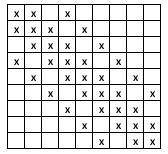
\includegraphics[width=0.2\linewidth]{matrix2D9x9}
	\end{center}
	\item The vector of vectors $a$ is used for the matrix $A$'s bands while $b$ is used for the right-hand side of $Ax=b$.
	
\end{itemize}

\vspace{1cm}
\noindent
\textbf{(Bonus)Part 4b.} Test the banded solver with the following system describing a 2D finite difference spatial discretization of the boundary value problem (BVP), 
$$
-\bnabla \dotp (\bnabla x) + x = 1,
$$
that results in the discrete set of equations, given the constant $N_c$,
\beq 
(4+h^2) x_{ij} 
- x_{i-1j} - x_{i+1j} - x_{ij-1} - x_{ij+1}
&= h^2 \\
\eeq 
\beq
x_{-1,j} &= 0 \quad x_{N_c,j} &= 0 \\
x_{i,-1} &= 0 \quad x_{i,N_c} &= 0 \\
\eeq
\beq 
h = \frac{1}{N_c}
\eeq 
The cell-wise index $ij$ maps to a single index as 
$$(i,j) \mapsto k \ : \ k = i + j N_c$$
which represents a lexicographical sorting of cells at $(x,y)$ index $(i,j)$. Consequently the $N_c{\times}N_c$ number of cells map to a system of equations where the matrix dimension is $N_c^2 {\times} N_c^2$ and the dimension of the vectors are $N_c^2{\times}1$.

%\begin{thebibliography}{1}
%	
%	\bibitem{LewisMiller} Lewis E.E., Miller W.F., {\em Computational Methods of Neutron Transport}, JohnWiley \& Sons, 1984
%	   
%\end{thebibliography}

%\newpage
%\begin{appendices}
%\section{First appendix}
%Put ``Lazy reader stuff here".
%\end{appendices}

\end{document}